\documentclass{article}

\usepackage{tikz}
\usetikzlibrary{calc}
\begin{document}
\begin{figure}
\tikzset{
tick/.style = {black, very thick}
}

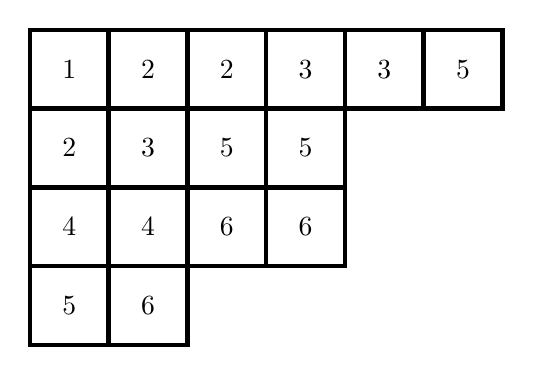
\begin{tikzpicture} % boxlength=1%ZEILE NR. 0 (von unten)

%ELEMENT IN SPALTE NR. 0 (von links)
\draw [ultra thick] (0,0) rectangle (1,1);
\node at ($(0.5,0.5)$) {$5$};

%ELEMENT IN SPALTE NR. 1 (von links)
\draw [ultra thick] (1,0) rectangle (2,1);
\node at ($(1.5,0.5)$) {$6$};




%ZEILE NR. 1 (von unten)

%ELEMENT IN SPALTE NR. 0 (von links)
\draw [ultra thick] (0,1) rectangle (1,2);
\node at ($(0.5,1.5)$) {$4$};

%ELEMENT IN SPALTE NR. 1 (von links)
\draw [ultra thick] (1,1) rectangle (2,2);
\node at ($(1.5,1.5)$) {$4$};

%ELEMENT IN SPALTE NR. 2 (von links)
\draw [ultra thick] (2,1) rectangle (3,2);
\node at ($(2.5,1.5)$) {$6$};

%ELEMENT IN SPALTE NR. 3 (von links)
\draw [ultra thick] (3,1) rectangle (4,2);
\node at ($(3.5,1.5)$) {$6$};




%ZEILE NR. 2 (von unten)

%ELEMENT IN SPALTE NR. 0 (von links)
\draw [ultra thick] (0,2) rectangle (1,3);
\node at ($(0.5,2.5)$) {$2$};

%ELEMENT IN SPALTE NR. 1 (von links)
\draw [ultra thick] (1,2) rectangle (2,3);
\node at ($(1.5,2.5)$) {$3$};

%ELEMENT IN SPALTE NR. 2 (von links)
\draw [ultra thick] (2,2) rectangle (3,3);
\node at ($(2.5,2.5)$) {$5$};

%ELEMENT IN SPALTE NR. 3 (von links)
\draw [ultra thick] (3,2) rectangle (4,3);
\node at ($(3.5,2.5)$) {$5$};




%ZEILE NR. 3 (von unten)

%ELEMENT IN SPALTE NR. 0 (von links)
\draw [ultra thick] (0,3) rectangle (1,4);
\node at ($(0.5,3.5)$) {$1$};

%ELEMENT IN SPALTE NR. 1 (von links)
\draw [ultra thick] (1,3) rectangle (2,4);
\node at ($(1.5,3.5)$) {$2$};

%ELEMENT IN SPALTE NR. 2 (von links)
\draw [ultra thick] (2,3) rectangle (3,4);
\node at ($(2.5,3.5)$) {$2$};

%ELEMENT IN SPALTE NR. 3 (von links)
\draw [ultra thick] (3,3) rectangle (4,4);
\node at ($(3.5,3.5)$) {$3$};

%ELEMENT IN SPALTE NR. 4 (von links)
\draw [ultra thick] (4,3) rectangle (5,4);
\node at ($(4.5,3.5)$) {$3$};

%ELEMENT IN SPALTE NR. 5 (von links)
\draw [ultra thick] (5,3) rectangle (6,4);
\node at ($(5.5,3.5)$) {$5$};







\end{tikzpicture}
\end{figure}
\end{document}

